\documentclass{tufte-handout}

\title{Section 2.2 Graphs of Functions}

\author[AW]{Ammon Washburn}

\usepackage{graphicx} % allow embedded images
  \setkeys{Gin}{width=\linewidth,totalheight=\textheight,keepaspectratio}
  \graphicspath{{graphics/}} % set of paths to search for images
\usepackage{amsmath}  % extended mathematics
\usepackage{booktabs} % book-quality tables
\usepackage{units}    % non-stacked fractions and better unit spacing
\usepackage{multicol} % multiple column layout facilities
\usepackage{lipsum}   % filler text
\usepackage{fancyvrb} % extended verbatim environments
  \fvset{fontsize=\normalsize}% default font size for fancy-verbatim environments

% Standardize command font styles and environments
\newcommand{\doccmd}[1]{\texttt{\textbackslash#1}}% command name -- adds backslash automatically
\newcommand{\docopt}[1]{\ensuremath{\langle}\textrm{\textit{#1}}\ensuremath{\rangle}}% optional command argument
\newcommand{\docarg}[1]{\textrm{\textit{#1}}}% (required) command argument
\newcommand{\docenv}[1]{\textsf{#1}}% environment name
\newcommand{\docpkg}[1]{\texttt{#1}}% package name
\newcommand{\doccls}[1]{\texttt{#1}}% document class name
\newcommand{\docclsopt}[1]{\texttt{#1}}% document class option name
\newenvironment{docspec}{\begin{quote}\noindent}{\end{quote}}% command specification environment

\newtheorem{mydef}{Definition}
\providecommand{\floor}[1]{\left \lfloor #1 \right \rfloor }

\begin{document}
\maketitle

\begin{abstract}
We will try to learn about graphs of functions and how to recognize that an equation or curve is a function
\end{abstract}
\section{Graphs}
\subsection{Curves}
\begin{mydef}
A graph of a function f with domain $A$ is the set of ordered pairs $(x,f(x))$ where $x \in A$
\end{mydef}

In other words the graph of f are the points (x,y) where y = f(x).  So the height of the graph is the value of f at x.

Linear functions can be made to look like $f(x) = mx+b$.  $m$ is the slope while $b$ is the y-intercept.  Constant functions look like $f(x) = b$
\subsection{Graphing with tables}
Consider the function and a table of some points from the graph

\begin{marginfigure}
  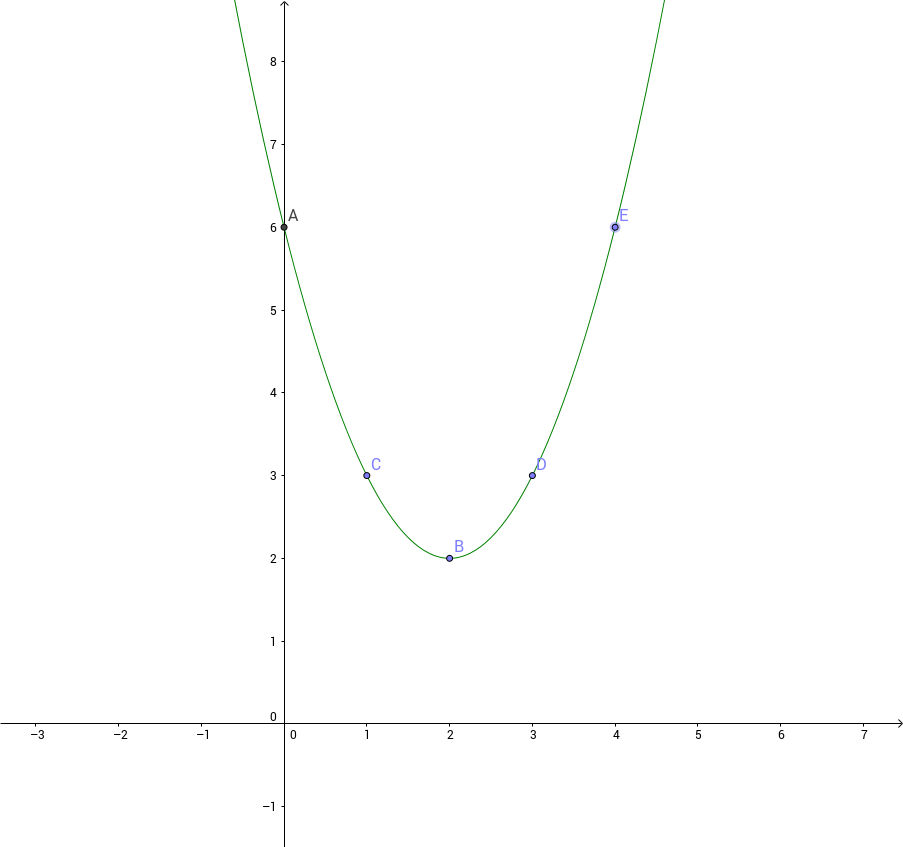
\includegraphics[width=\linewidth]{2-2GraphTable.png}
  \caption{You can use a few points to plot the outline of a function and you can usually fill in the dots.}
  \label{fig:table}
\end{marginfigure}

\[t(x) = (x-2)^2 + 2\]

\begin{table}
\centering
	\begin{tabular}{c || c | c | c | c | c}
		x & 0 & 1 & 2 & 3 & 4 \\
		\hline
		t(x) & 6 & 3 & 2 & 3 & 6 \\
	\end{tabular}
\end{table}

Graphing these points on a Cartesian plane you can start to see what the function should look like.  You can guess because this function should be continuous or have no "holes" or "jumps".  

Consider the greatest integer function or floor function $h(x) = \floor{x}$ (or in textbook $h(x) = [[x]]$).  This function is not continuous because it jumps every time you hit an integer.

\begin{table}
	\centering
	\begin{tabular}{c || c | c | c | c}
		x & -1.5 & 0.9999999 & 1 & 1.0000001 \\
		\hline
		h(x) & -2 & 0 & 1 & 1 \\
	\end{tabular}
    \caption{There is jump from as you go past x = 1}
\end{table}

What is $h(1)$? It is the greatest integer less than or \textit{equal} to 1.  Since 1 is in an integer then it is 1.

\begin{marginfigure}
	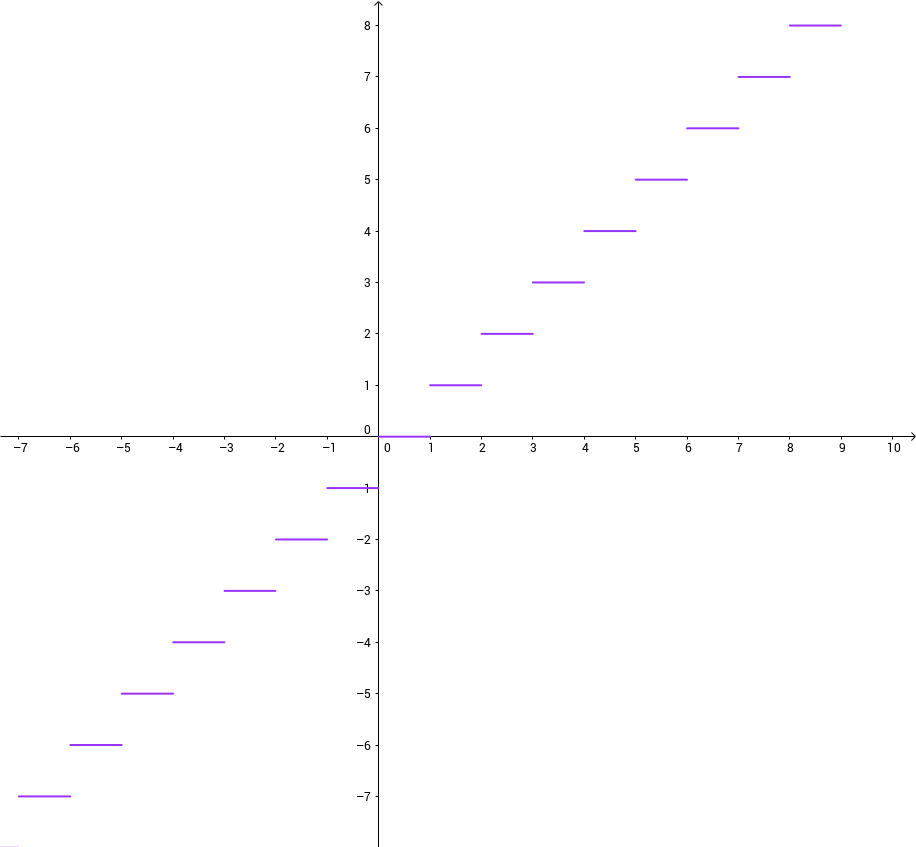
\includegraphics[width=\linewidth]{2-2floor.png}
	\caption{The greatest integer looks for the closest integer that is below or equal to your input.}
    \label{fig:floor}
\end{marginfigure}

\subsection{Graphing with your calculator}

Try graphing $y = x^3 -10x^2-10$ on your calculator.  When graphing with your calculator be sure your window is in the right spot.  ZStandard puts in the normal window.  ZoomFit (the number 0) will try to put the graph in the middle.  The window section will allow you to specify the window you want.  Put [-10,30] for xmin and xmax and try [-2010,17990] for ymin and ymax and you will see the function.

You also have to take what your calculator gives you with a grain of salt.  Try graphing $y = \log(x-1) + 5$.  It looks like the graphs cuts off around one but really it keeps going down.

\section{Determining whether an equation, graph, or table is a function}
\subsection{Vertical Line test}
If you have a graph given to you then you can determine if the graph represents a function by using the vertical line test.  This means you imagine a vertical line that is moving along.  If at any time the vertical line touches two points on the graph, then it is not a function.

\begin{marginfigure}
	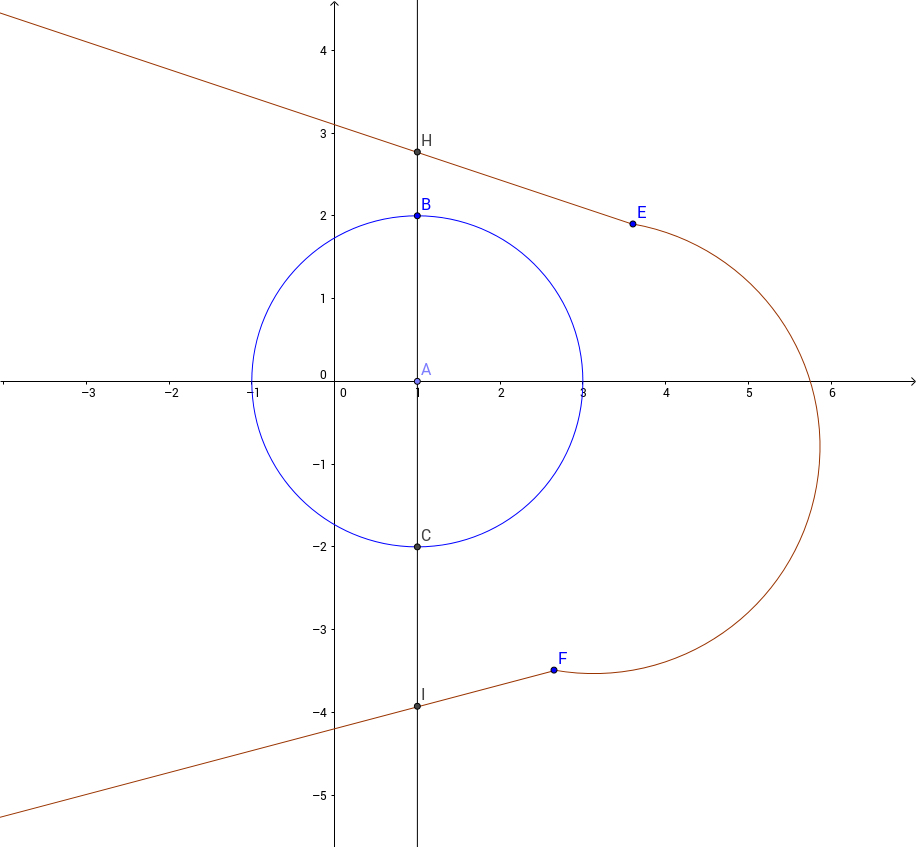
\includegraphics[width=\linewidth]{2-2VertLineTest.png}
    \caption{Notice that at points B and C that the vertical line touches two points on the circle.  Also the vertical line touches two points on the graph around the circle so it is also not a function}
\end{marginfigure}

\subsection{Tables as function}
If inputs appear twice but with different outputs then it is not a function.  In each of the following examples decide if y is a function of x. Answers are no, yes, yes.
\begin{table}
\centering
\begin{tabular}{c || c | c | c | c}
x & -2 & 3 & -1 & 3 \\
\hline
y & 2 & 4 & 6 & 7 \\
\end{tabular}
\quad
\begin{tabular}{c || c | c | c | c}
x & 1 & 2 & 3 & 4 \\
\hline
y & 1 & 1 & 1 & 1 \\
\end{tabular}
\quad
\begin{tabular}{c || c | c | c | c}
x & -1 & -2 & -3 & -1 \\
\hline
y & 2 & 4 & 6 & 2 \\
\end{tabular}
\end{table}

\subsection{Equations as functions}
If you are given an equation with $y$ and $x$ you can solve for $y$ and see if one value of $x$ will give you one value of $y$.

a) $y^2 + 4x^2 = 16$ \hspace{1 cm} b) $ yx-1 = x + y$

a) simplifies to $ y = \pm \sqrt[]{16 - 4x^2}$.  This does not represent $y$ as a function of $x$ because there are two different possible $y$ values for each $x$

b) simplifies to $ y = \frac{x+1}{x-1}$. This does represent $y$ as a function of x however we can see that $x=1$ is not in the domain of $y(x)$.

\section{Quiz}
You can use your graphing calculator on this part.  Be sure in include the open and closed dots as well as be sure you put domain and range in interval notation with proper parenthesis and brackets.










\end{document}